I henhold til geometriske fremstillinger af lineære programmeringsproblemer er det nødvendigt at definere en række begreber.
Disse er \textit{hyperplan}, \textit{halvrum} og \textit{polytop}.
%
\begin{defn}{}{Polytop}
Lad $A$ være en $m \times n$ matrix, og lad $\mathbf{b}$ være en vektor i  $\R^m$.
En \textbf{polytop} er en mængde, der kan beskrives som 
\begin{align*}
\{x\in \R^n \mid A\mathbf{x}\geq b\}.
\end{align*}
%
\end{defn}
\noindent
%
Som det fremgår fra definitionen, er en polyetop således mængden af mulige løsninger $\mathbf{x}$ af et ligningssystem.
Det gælder endvidere, at en mængde af formen $ \{x \in \R^n \mid A\textbf{x}=b,x \geq 0 \}$, hvilket kaldes en \textit{polytop på standardform}. 
% Kommentar til at der her er derfor det er rellevant og at det vil blive uddybet senere 
% Eventuelt med et eksempel 
%lidt forskellige muligheder her, enten kan det relateres til simplex eller blive introduceret her
%
Det gælder endvidere for polytoper at disse både kan være \textit{begrænsede} og \textit{ubegrænsede}.
%
\begin{defn}{}{}
En mængde $S \subset \R^n$ er \textbf{begrænset} såfremt der eksister en konstant $c$, hvorom det gælder, at den absolutte værdi af alle komponenter i alle elementer i $S$ er $\leq c$. 
Såfremt en sådan konstant ikke eksisterer er mængden \textbf{ubegrænset}. 
\end{defn}
\noindent
%
%alternativt værdien af ..... $\leq k$ eller $\geq$
%
I henhold til lineære programmeringsproblemer vil dette ofte være begrænset.
% Dette er eksempelvis tilfældet, hvis problemet er af en sådan karakter, at ingen af variabelene i karakterligningen kan have negative værdier.
%er det rigtigt det jeg skriver i ovenstående?
Ligeledes er det en fordel at definere polytope, der er begrænset af kun én lineær betingelse. 
%
%skal der laves en definition på et polyede?
%
\begin{defn}{}{}
Lad $\mathbf{a}$ være en vektor i $\R^n$, hvor $\mathbf{a} \neq \mathbf{0}$ og lad $b$ være en skalar.
\begin{enumerate}[label=(\alph*)]
\item Mængden $\{x \in \R^n \mid \mathbf{a}^T \mathbf{x}=b\}$ kaldes et \textbf{hyperplan}.
\item Mængden $\{x \in \R^n \mid \mathbf{a}^T \mathbf{x} \geq b\}$ kaldes et \textbf{halvrum}.
\end{enumerate}
\end{defn}
\noindent
%
Det gælder her, at hyperplanet er grænsen for et tilsvarende halvrum.
I $\R^2$ vil hyperplanet således være en ret linje, som afskære en del af rummet, og der vil dermed være et halvrum på hvad side af hyperplanet.
På figur \ref{fig:Graf123} ses et udsnit af hyperplanet, som afskærer et halvrum markeret med gråblå og et halvrum markeret med orangerød. 

%%%%%%%%%%%%%%%%%%%%%%%%%%%%%%%%
%%% Flot graf alla Julie     %%%
%%%%%%%%%%%%%%%%%%%%%%%%%%%%%%%%
\begin{center}
\begin{tikzpicture}
% Den øverste linje
\draw[name path=b,-, white, thick] (0,3.5) -- (6,3.5);
%
% Den nederste linje
\draw[name path=c,-, white, thick] (0,-1) -- (6,-1);
%
% Den mellemste linje
\draw[name path=a,-, white, thick] (0,0) -- (6,3);
%
% Farvning 
\tikzfillbetween [of=a and b]{myblue!5}
\tikzfillbetween [of=a and c]{myred!5}
%
% Linjen mellem 
\draw[-, black, very thick] (0,0) -- (6,3);
\draw[->, black, thick] (2.4,1.2) -- (2,2);
\filldraw[black] (0.2,-0.3) circle (0pt) node[anchor=west] {$\mathbf{a}^T \mathbf{x}=b$};
\filldraw[black] (3,2.6) circle (0pt) node[anchor=west] {$\mathbf{a}^T \mathbf{x} > b$};
\filldraw[black] (3,1.3) circle (0pt) node[anchor=west] {$\mathbf{a}^T \mathbf{x} < b$};
\filldraw[black] (1.6,2.2) circle (0pt) node[anchor=west] {$\mathbf{a}$};
\end{tikzpicture}
  \captionof{figure}{Et hyperplan og to halvrum, markeret med henholdsvis gråblå for $\mathbf{a}^T \mathbf{x} < b$ og orangerød for $\mathbf{a}^T \mathbf{x} > b$.}
  \label{fig:Graf123}
\end{center}

%%%%%%%%%%%%%%%%%%%%%%%%%%%%%%%%
%%% Flot graf alla Julie     %%%
%%% Soooom ikke er færdig    %%%
%%%%%%%%%%%%%%%%%%%%%%%%%%%%%%%%
\begin{center}
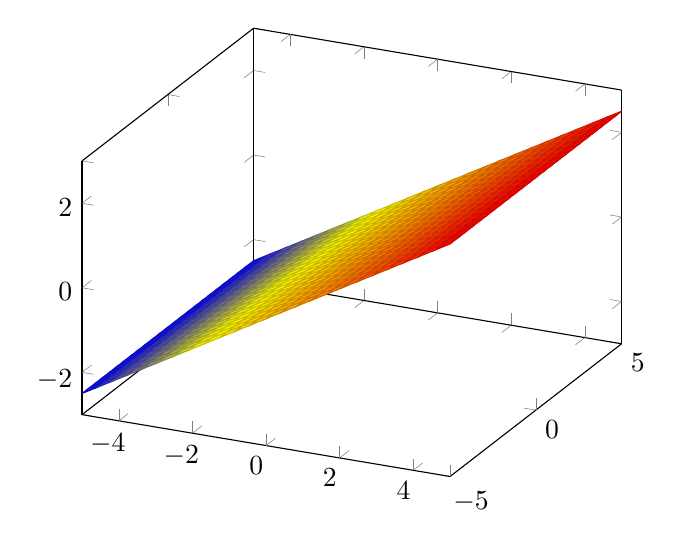
\begin{tikzpicture}
\begin{axis}
\addplot3[
    surf,
]
{0.5*x};
\end{axis}
\end{tikzpicture}
  \captionof{figure}{FUCK DET HER LORT XD}
  \label{fig:NEJ}
\end{center}
% 

%Et polyhedron er derfor en samling af polyeder der til sammen skaber en geometrisk figur i et givet vektorrum.
%ligeldes bør der nævnes noget med at a står vinkelret på linjen 

\begin{thm}{}{}
Lad $\mathbf{a}$ være en vektor i $\R^n$, hvor $\mathbf{a} \neq \mathbf{0}$
\end{thm}